\section{Clustering}\label{sec:clustering}

\begin{frame}
    \frametitle{Clustering}

    \begin{itemize}
        \item<1-> Algoritmos de aprendizaje no supervisado que agrupan los elementos de una colección de datos en conjuntos (\textbf{clusters}).
        \item<2-> Simplificar la estructura del conjunto de datos.
        \item<3-> Encontrar grupos de especial significación.
    \end{itemize}

    \begin{itemize}
        \item<3-> ¿Qué constituye un cluster?
        \item<4-> ¿Cómo hallarlos eficientemente?
    \end{itemize}

\end{frame}

\begin{frame}
    \frametitle{Clustering Particional}

    \begin{block}{K-Means}
        \begin{enumerate}
            \item<2-> Seleccionar $K$ puntos como \textit{centroides} iniciales.
            \item<3-> Formar $K$ clusters asignando cada punto al centroide más próximo.
            \item<4-> Recomputar el centroide de cada cluster.
            \item<5-> Repetir los pasos 2 y 3 hasta que se cumpla cierto \textit{criterio de convergencia}.
        \end{enumerate}
    \end{block}

    \begin{itemize}
        \item<6-> Minimizar la \textbf{Suma de Errores Cuadráticos} (SSE).
        \item<7-> Centroides que son la media de sus clusters minimizan la SSE\@.
    \end{itemize}

\end{frame}

\begin{frame}

    \begin{block}{Selección de centroides iniciales}
        \begin{itemize}
            \item<2-> aleatoria
            \item<3-> clustering jerárquico hasta formar $K$ clusters y tomar sus centoides
            \item<4-> \textbf{K-Means++}
        \end{itemize}
    \end{block}

    \pause
    \begin{block}{Estimación del número de clusters}
        \begin{itemize}
            \item<5-> Criterio de Información de Akaike: $K=argmin_{K}[SSE(K)+2M K]$
            \item<6-> Coeficiente de Silueta
            \item<7-> Índice de Calinski-Harabasz
        \end{itemize}
    \end{block}

\end{frame}

\begin{frame}
    \frametitle{Clustering Jerárquico}

    \begin{itemize}
        \item<2-> \textbf{Aglomerativos}: Cada punto comienza en un cluster propio.
        Iterativamente se van uniendo hasta alcanzar un único cluster.
        \item<3-> \textbf{Divisivos}: Todos los puntos pertenecen a un mismo cluster inicial.
        De forma iterativa se separa un cluster en dos, hasta obtener clusters de un único punto.
    \end{itemize}

\end{frame}

\begin{frame}

    \begin{block}{Clustering Jerárquico Aglomerativo}
        \begin{enumerate}
            \item<2-> Computar la matriz de proximidad si es necesario.
            \item<3-> Unir los dos clusters \textbf{más próximos}.
            \item<4-> Actualizar la matriz de proximidad en correspondencia con las distancias entre el nuevo cluster y los ya existentes.
            \item<5-> Repetir los pasos 2 y 3 hasta que \textit{exista solamente un cluster}.
        \end{enumerate}
    \end{block}

    \begin{itemize}
        \item<6-> \textit{Single link}.
        \item<7-> \textit{Complete link}.
        \item<8-> \textit{Group averaged} y \textit{Centroid-based}.
        \item<9-> \textit{Método de Ward}.
    \end{itemize}

\end{frame}

\begin{frame}
    \frametitle{Clustering Basado en Densidad}

    \begin{figure}[!h]
        \centering
        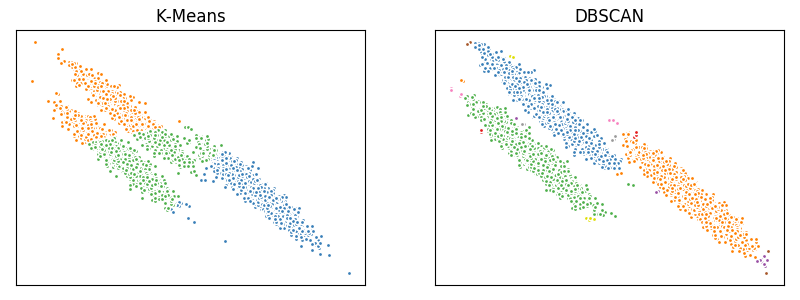
\includegraphics[width=\textwidth]{kmeans-dbscan.png}
    \end{figure}

    {\footnotesize
    Resultados de los algoritmos K-Means y DBSCAN ejecutados sobre un conjunto de datos que sigue una distribución \textit{anisotrópica}.
    }

\end{frame}

\begin{frame}
    \frametitle{Clustering Basado en Densidad}

    \begin{block}{Densidad de un punto}
        Cantidad de puntos localizados alrededor de este en un radio, $Eps$, específico.
        El propio punto es incluido en el conteo.
    \end{block}

    \pause
    \alert{El valor del radio es determinante en la densidad de un punto.}

    \pause
    \begin{figure}[!h]
        \centering
        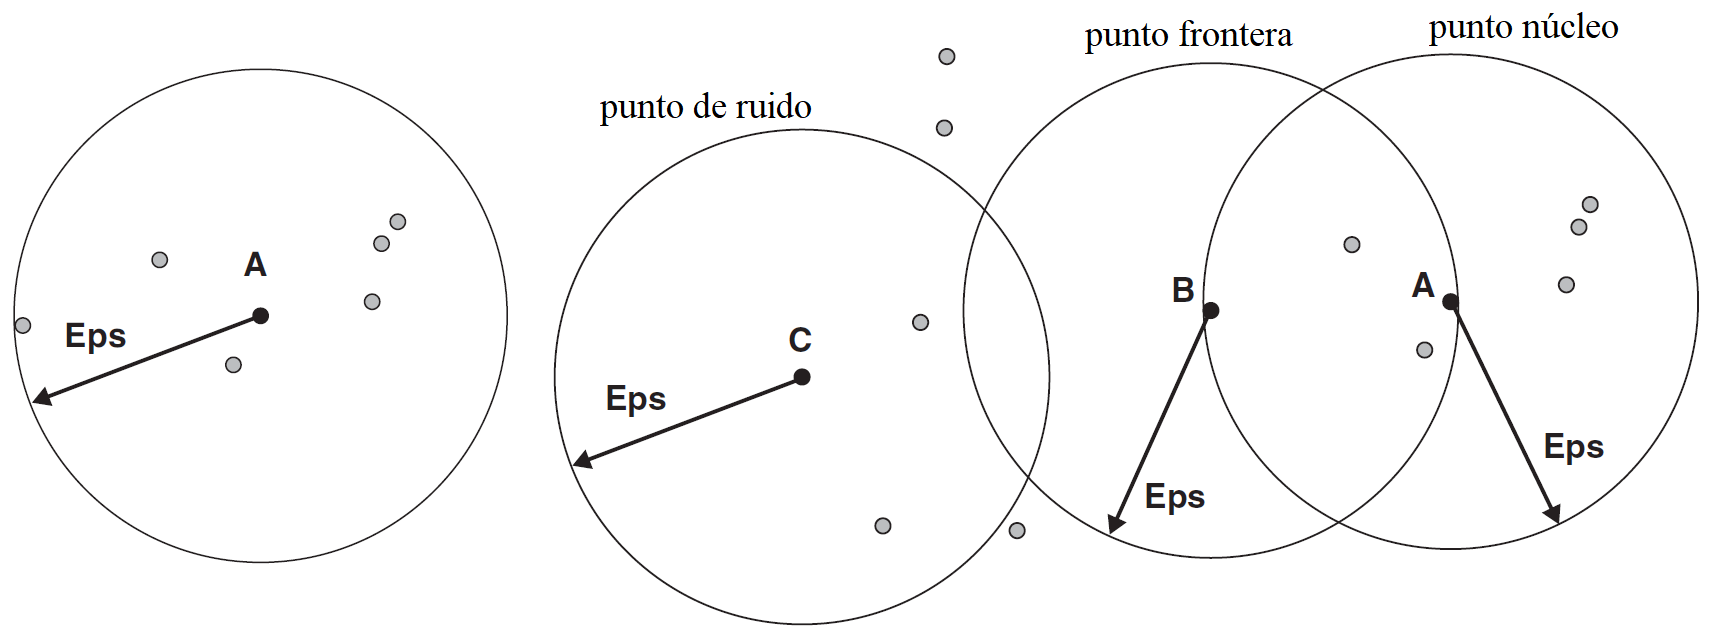
\includegraphics[width=0.8\textwidth]{dbscan.png}
    \end{figure}
\end{frame}

\begin{frame}
    \frametitle{Clustering Basado en Densidad}

    \begin{block}{DBSCAN}
        \begin{enumerate}
            \item<2-> Etiquetar todos los puntos como \textit{núcleo}, \textit{frontera} o \textit{ruido}.
            \item<3-> Eliminar los puntos de ruido.
            \item<4-> Añadir una arista entre todo par de puntos núcleos que se encuentren a una distancia menor o igual que $Eps$.
            \item<5-> Convertir cada componente conexa del grafo resultante en un cluster.
            \item<6-> Asignar cada punto frontera a uno de los clusters de los puntos núcleos asociados a este.
        \end{enumerate}
    \end{block}

\end{frame}

\begin{frame}

    Selección de parámetros para DBSCAN:

    \begin{itemize}
        \item<2-> \textbf{$k$-distancia de un punto}: Distancia al $k$-ésimo punto más cercano a este.
        \item<3-> Los valores de la k-distancias para puntos que pertenezcan a algún cluster no mostrarán un rango de valores muy amplio.
        \item<4-> Para puntos que no pertenezcan a ningún cluster, es decir, de ruido, el valor sí estará situado muy por encima del rango antes mencionado.
        \item<5-> Si se observan en una gráfica las $k$-distancias ordenadas de menor a mayor, el punto de inflexión corresponderá al valor $Eps$.
        \item<6-> $MinPts$ será el $k$ seleccionado para calcular las $k$-distancias.
    \end{itemize}

\end{frame}

\begin{frame}

    \begin{figure}[!h]
        \centering
        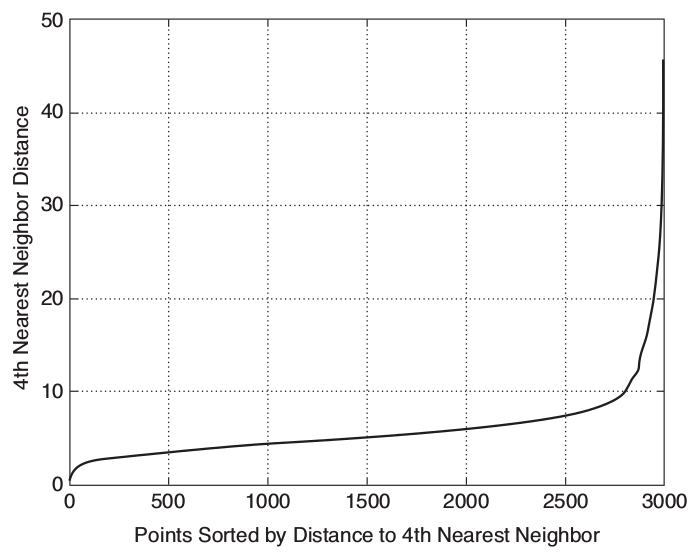
\includegraphics[width=0.7\textwidth]{dbscan-k-dist.png}
    \end{figure}

    {\footnotesize
    Representación de los puntos de un conjunto de datos ordenados por su $k$-distancia ($k=4$).
    }

\end{frame}

\begin{frame}
    \frametitle{Clustering Basado en Densidad}

    \begin{figure}[!h]
        \centering
        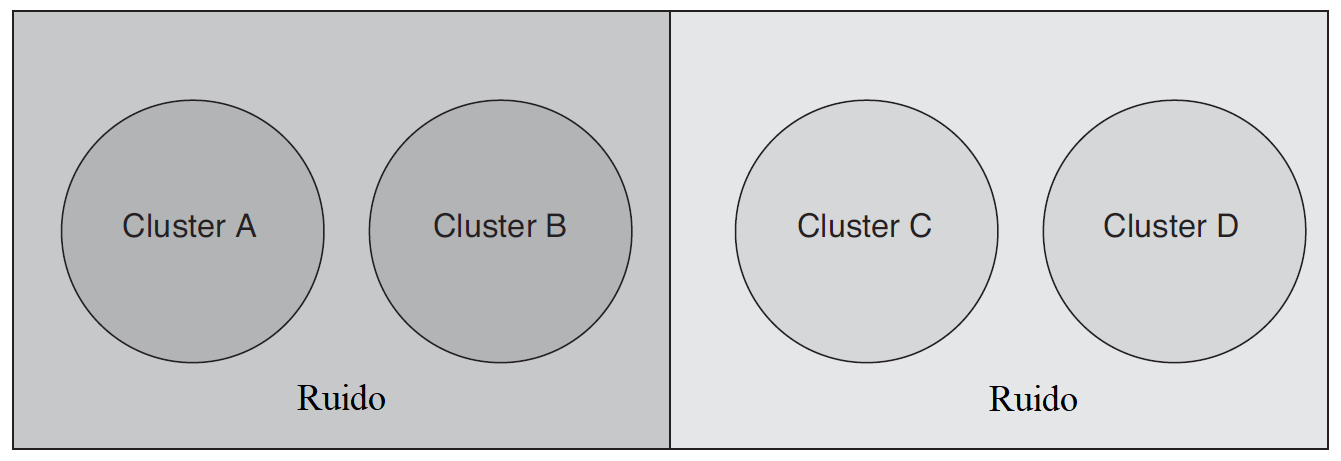
\includegraphics[width=\textwidth]{density-issues.png}
    \end{figure}

    {\footnotesize
    Cuatro clusters en un entorno de ruido.
    Los tonos de gris más oscuros indican mayores densidades.
    }

\end{frame}

\begin{frame}
    \frametitle{Clustering Basado en Densidad}

    \begin{block}{HDBSCAN}
        \begin{enumerate}
            \item<2-> Transformar el espacio en correspondencia con la densidad/dispersión de los puntos.
            \item<3-> Computar el árbol abarcador de costo mínimo correspondiente al grafo completo ponderado por las distancias halladas.
            \item<4-> Construir una jerarquía de componentes conexas (clusters).
            \item<5-> Condensar la jerarquía a partir de un tamaño mínimo para los clusters.
            \item<6-> Extraer los clusters estables del árbol condensado.
        \end{enumerate}
    \end{block}

\end{frame}

\begin{frame}

    \begin{block}{Distancia de alcanzabilidad mutua}
        \begin{equation*}
            d_{mreach}(a,b)=\max(dist_k(a), dist_k(b), dist(a,b))
        \end{equation*}
    \end{block}

    \begin{figure}[!h]
        \centering
        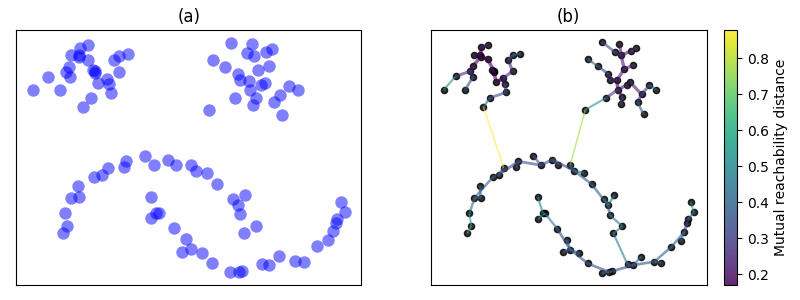
\includegraphics[width=\textwidth]{hdbscan-dataset+mst.png}
    \end{figure}

\end{frame}

\begin{frame}

    Se eliminan todas las aristas del grafo y se las añade en orden ascendente según su peso, cada componente conexa que unen constituye el cluster padre de los clusters correspondientes en la jerarquía.

    \begin{figure}[!h]
        \centering
        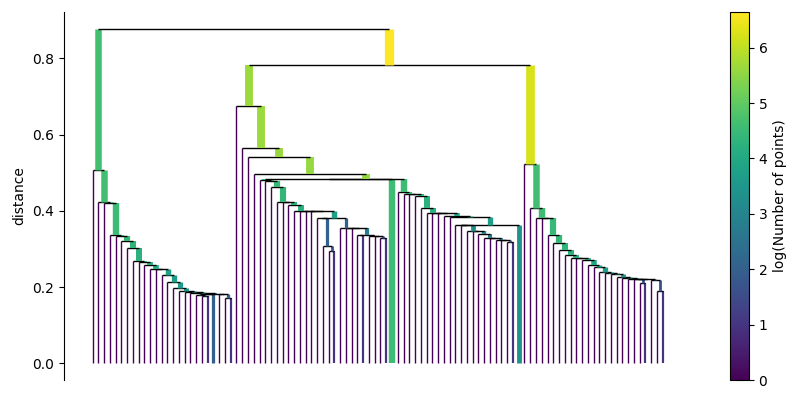
\includegraphics[width=0.8\textwidth]{hdbscan-hierarchy.png}
    \end{figure}

\end{frame}

\begin{frame}

    Generalmente al dividirse un cluster, solo se separan unos pocos puntos mientras el grueso de sus elementos permanecen en el otro cluster hijo.

    \pause
    {\footnotesize
    \begin{columns}
        \column{0.2\textwidth}

        \begin{equation*}
            \lambda = \frac{1}{d_{mreach}}
        \end{equation*}

        \column{0.8\textwidth}

        \begin{itemize}
            \item $\lambda_{birth}$: Valor de $\lambda$ en que surge el nodo.
            \item $\lambda_{death}$: Valor de $\lambda$ en que el nodo se divide.
            \item $\lambda_p$: Valor de $\lambda$ en que se elimina el punto $p$.
        \end{itemize}

    \end{columns}
    }

    \begin{enumerate}
        \item<3-> Se toma como solución inicial el conjunto de nodos hojas del árbol condensado.
        \item<4-> Iterativamente se recorre el árbol hacia arriba, comparando el $\lambda$ de cada nodo con la suma de sus hijos:
        \begin{itemize}
            \item<5-> si es menor, se sustituye por la suma
            \item<5-> si es mayor, se mantiene, y los hijos son reemplazados por el padre en la solución
        \end{itemize}
    \end{enumerate}

\end{frame}

\begin{frame}

    \begin{figure}[!h]
        \centering
        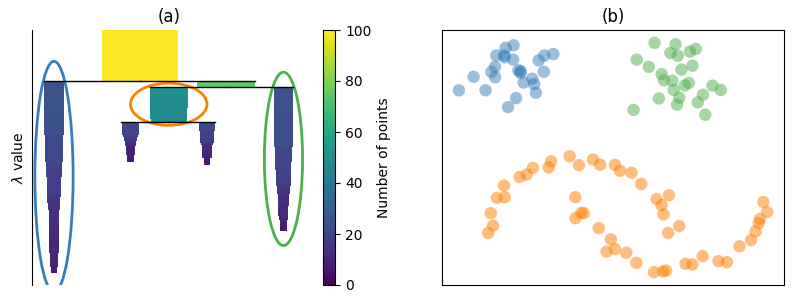
\includegraphics[width=\textwidth]{hdbscan-hierarchy-condensed+results.png}
    \end{figure}

\end{frame}

\begin{frame}
    \frametitle{Clustering Basado en Probabilidades}

    \begin{block}{Combinación de modelos}
        \begin{equation*}
            p(x_i)=\sum_{k=1}^{K}{\pi_k p(x_i|\theta_k)}
        \end{equation*}
    \end{block}

    \begin{itemize}
        \item $\theta_k$: conjunto de parámetros específicos del modelo $k$.
        \item $p(x_i|\theta_k)$: función de densidad.
    \end{itemize}

\end{frame}

\begin{frame}

    \begin{block}{Gaussian Mixture Model (GMM)}
        \begin{itemize}
            \item<2-> Asume que los puntos del conjunto de datos son generados mediante la combinación de un número finito de distribuciones normales con parámetros desconocidos (\textit{media} y \textit{covarianza}).
            \item<3-> K-Means generalizado para incorporar información sobre la covarianza de los datos.
        \end{itemize}
    \end{block}

    \pause
    \begin{block}{Método de máxima verosimilitud}
        \begin{equation*}
            l(\Theta|X) = \sum_{i=1}^{N}{\log{\sum_{k=1}^{K}{\pi_k \mathcal{N}(x_i|\mu_k,\Sigma_k)}}}
        \end{equation*}
    \end{block}

    \pause
    \alert{EXPECTATION-MAXIMIZATION}

\end{frame}

\begin{frame}
    \frametitle{Clustering Basado en Grafos}

\end{frame}